\documentclass[border={20.000000bp 20.000000bp 20.000000bp 20.000000bp}, 11pt]{standalone}
%

\usepackage{tikz}
\usepackage{xcolor}
\usetikzlibrary{shapes.misc}
\usetikzlibrary{backgrounds}

\definecolor{dotColorA}{HTML}{222222}
\definecolor{dotColorB}{HTML}{222222}
\definecolor{dotColorC}{HTML}{222222}

\definecolor{labelBgColorA}{HTML}{222222}
\definecolor{labelBgColorB}{HTML}{222222}
\definecolor{labelBgColorC}{HTML}{222222}

\definecolor{labelTextColorA}{HTML}{FFFFFF}
\definecolor{labelTextColorB}{HTML}{FFFFFF}
\definecolor{labelTextColorC}{HTML}{FFFFFF}

\definecolor{linkColorA}{HTML}{222222}
\definecolor{linkColorB}{HTML}{222222}
\definecolor{linkColorC}{HTML}{222222}

\def\textA{Minimal}
\def\textB{Working}
\def\textC{Example}

\begin{document}
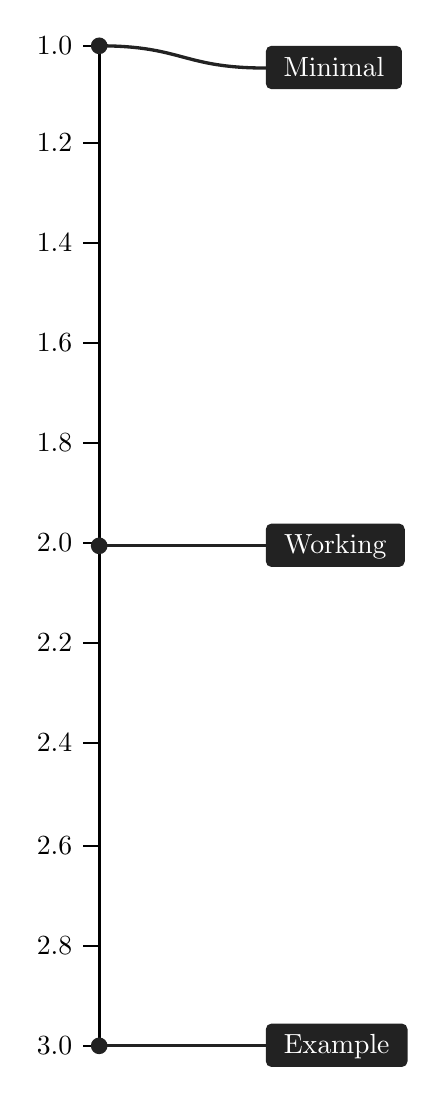
\begin{tikzpicture}[x=1bp,y=-1bp]

% shift for the margin
\begin{scope}[shift={(20, 20)}]
% main layer
\begin{scope}[shift={(0, 0)}]
% axis
\begin{scope}
\draw[very thick] (0, 0) -- (0, 360);
\end{scope}

% axis layer
\begin{scope}
\begin{scope}[shift={(0, 0)}]
\draw[thick] (0, 0) -- (-6pt, 0)
node[anchor=east] {1.0};
\end{scope}
\begin{scope}[shift={(0, 35)}]
\draw[thick] (0, 0) -- (-6pt, 0)
node[anchor=east] {1.2};
\end{scope}
\begin{scope}[shift={(0, 71)}]
\draw[thick] (0, 0) -- (-6pt, 0)
node[anchor=east] {1.4};
\end{scope}
\begin{scope}[shift={(0, 107)}]
\draw[thick] (0, 0) -- (-6pt, 0)
node[anchor=east] {1.6};
\end{scope}
\begin{scope}[shift={(0, 143)}]
\draw[thick] (0, 0) -- (-6pt, 0)
node[anchor=east] {1.8};
\end{scope}
\begin{scope}[shift={(0, 179)}]
\draw[thick] (0, 0) -- (-6pt, 0)
node[anchor=east] {2.0};
\end{scope}
\begin{scope}[shift={(0, 215)}]
\draw[thick] (0, 0) -- (-6pt, 0)
node[anchor=east] {2.2};
\end{scope}
\begin{scope}[shift={(0, 251)}]
\draw[thick] (0, 0) -- (-6pt, 0)
node[anchor=east] {2.4};
\end{scope}
\begin{scope}[shift={(0, 288)}]
\draw[thick] (0, 0) -- (-6pt, 0)
node[anchor=east] {2.6};
\end{scope}
\begin{scope}[shift={(0, 324)}]
\draw[thick] (0, 0) -- (-6pt, 0)
node[anchor=east] {2.8};
\end{scope}
\begin{scope}[shift={(0, 360)}]
\draw[thick] (0, 0) -- (-6pt, 0)
node[anchor=east] {3.0};
\end{scope}
\end{scope}

% link layer
\begin{scope}
\draw[color=linkColorA, very thick] (0.00000000, 0.00000000) .. controls
(30.00000000, 0.00000000) and (30.00000000, 8.00000000) .. (60.00000000, 8.00000000);
\draw[color=linkColorB, very thick] (0.00000000, 180.00000000) .. controls
(30.00000000, 180.00000000) and (30.00000000, 180.00000000) .. (60.00000000, 180.00000000);
\draw[color=linkColorC, very thick] (0.00000000, 360.00000000) .. controls
(30.00000000, 360.00000000) and (30.00000000, 360.00000000) .. (60.00000000, 360.00000000);
\end{scope}

% label layer
\begin{scope}
\begin{scope}[shift={(60, 0)}]
\fill[color=labelBgColorA, rounded corners=2pt]
(0, 0) rectangle (49, 15.60416) node[midway, yshift=-.75bp, anchor=center, text=labelTextColorA] {\strut \textA};
\end{scope}
\begin{scope}[shift={(60, 172)}]
\fill[color=labelBgColorB, rounded corners=2pt]
(0, 0) rectangle (50, 15.60416) node[midway, yshift=-.75bp, anchor=center, text=labelTextColorB] {\strut \textB};
\end{scope}
\begin{scope}[shift={(60, 352)}]
\fill[color=labelBgColorC, rounded corners=2pt]
(0, 0) rectangle (51, 15.60416) node[midway, yshift=-.75bp, anchor=center, text=labelTextColorC] {\strut \textC};
\end{scope}
\end{scope}

% dots
\begin{scope}
\draw node [circle, inner sep=0pt, minimum size=6bp, 
fill=dotColorA] at (0, 0.000000) {};
\draw node [circle, inner sep=0pt, minimum size=6bp, 
fill=dotColorB] at (0, 180.000000) {};
\draw node [circle, inner sep=0pt, minimum size=6bp, 
fill=dotColorC] at (0, 360.000000) {};
\end{scope}

\end{scope}
\end{scope}
\end{tikzpicture}
\end{document}